\documentclass[11pt]{beamer}

\usetheme{metropolis}

\usepackage{graphicx}
\usepackage{physics}
\usepackage{adjustbox}
\usepackage{caption}
\usepackage{chemformula}
\usepackage{quoting}
\usepackage[style=chem-angew,backend=bibtex]{biblatex}
\bibliography{references}
%
% Choose how your presentation looks.
%
% For more themes, color themes and font themes, see:
% http://deic.uab.es/~iblanes/beamer_gallery/index_by_theme.html
%
\mode<presentation>
{
  \usetheme{default}      % or try Darmstadt, Madrid, Warsaw, ...
  \usecolortheme{default} % or try albatross, beaver, crane, ...
  \usefonttheme{default}  % or try serif, structurebold, ...
  \setbeamertemplate{navigation symbols}{}
  \setbeamertemplate{caption}[numbered]
  \setbeamerfont{footnote}{size=\tiny}
} 

\usepackage[english]{babel}
\usepackage[utf8]{inputenc}
\graphicspath{{image/}}

\AtBeginSection[]{
\begin{frame}{Outline}
  \tableofcontents[currentsection]
\end{frame}
}

\title{Chapter 6: Quantities in Chemical Reactions}
\institute{Chemistry Department, Cypress College}
\date{October 10, 2022}

\begin{document}

\begin{frame}
  \titlepage
\end{frame}

\begin{frame}{Class Annoucements}
  \textbf{Lab}
  \begin{itemize}
  \item Experiment 12 - Single Displacement Reactions
  \item Recall indications for chemical reaction (color, solids,
    temp, etc.)
  \item Week 5 Lab assignments graded
  \item Reminder - Need $70\%$ of laborator points to pass the course
  \end{itemize}
  
  \textbf{Lecture}
  \begin{itemize}
  \item Finally graded homework 3 and go over homework 4 (EC for
    students who present)
  \item Finish up Ch 6 and worksheet 7; begin discussion on Ch 7
    - Electronic Structure of the Atom
  \item Quiz and Homework assignment released Fri, Oct 14th at 3pm
  \end{itemize}
\end{frame}

\section{Energy Changes}

\begin{frame}{Global Energy Consumption}
  \centering
  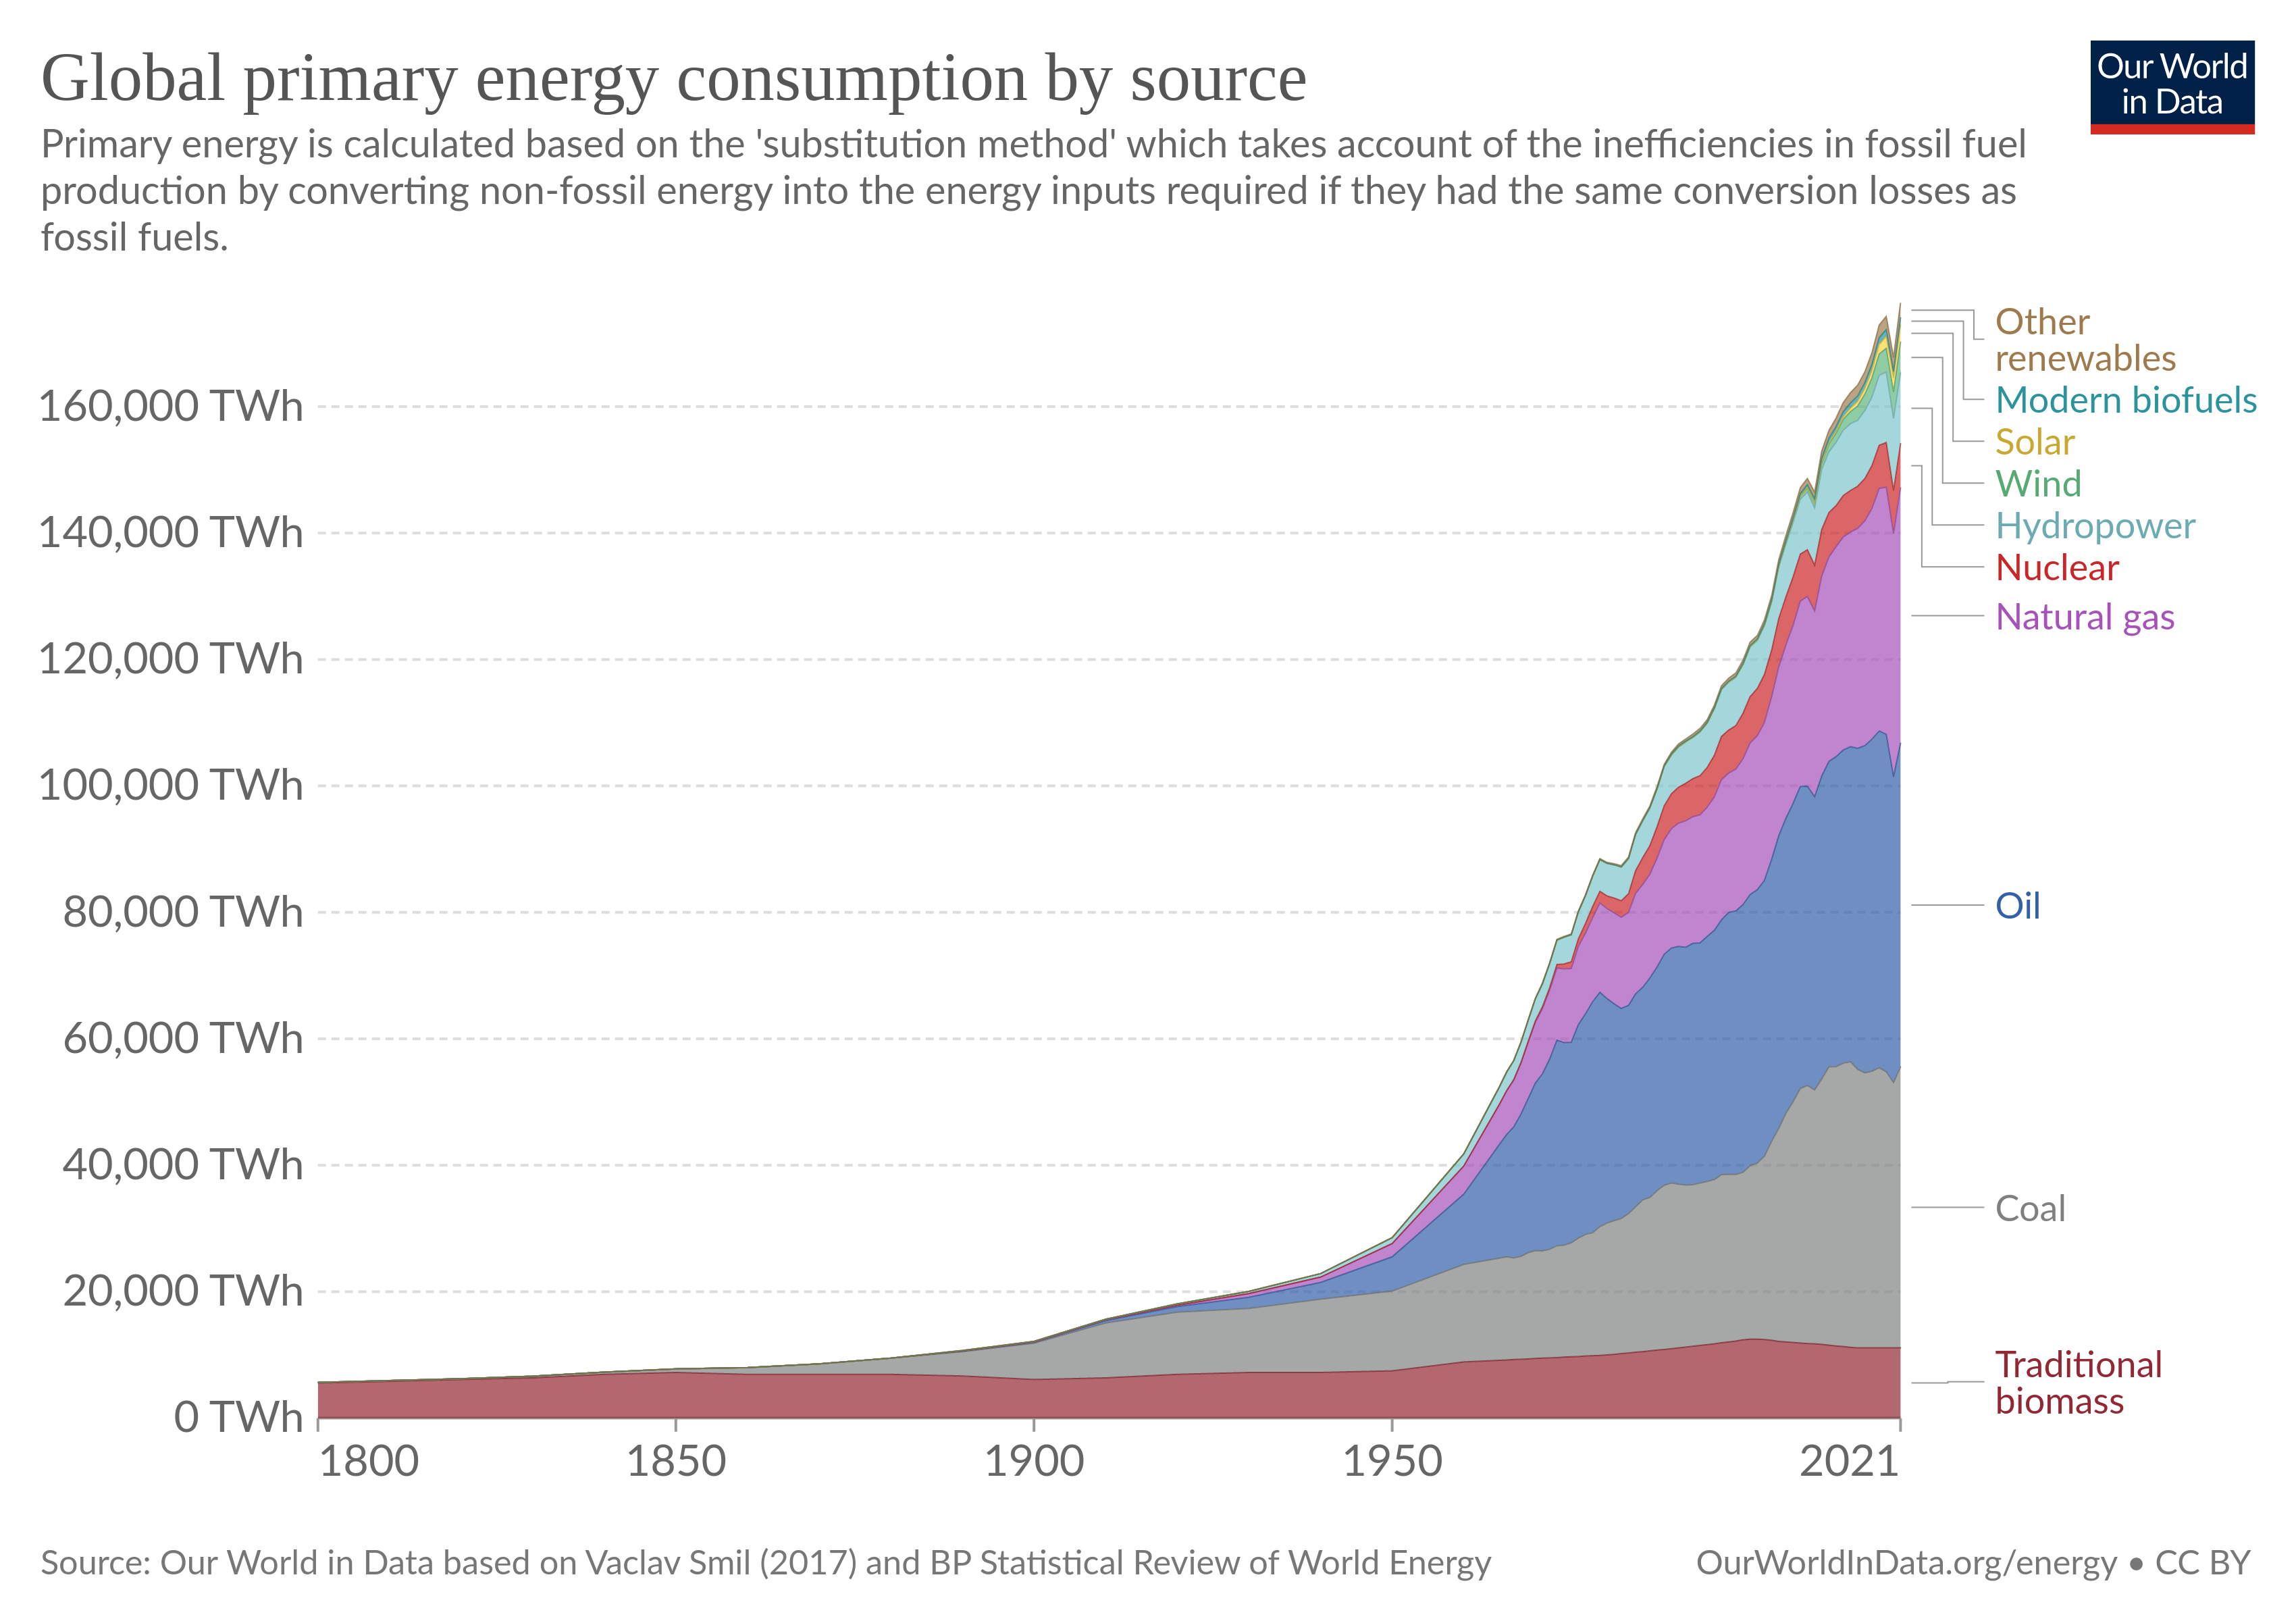
\includegraphics[width=\linewidth]{global_energy}
\end{frame}

\subsection{Law of Conservation of Energy}

\begin{frame}{Law of Conservation of Energy}
  \begin{center}
    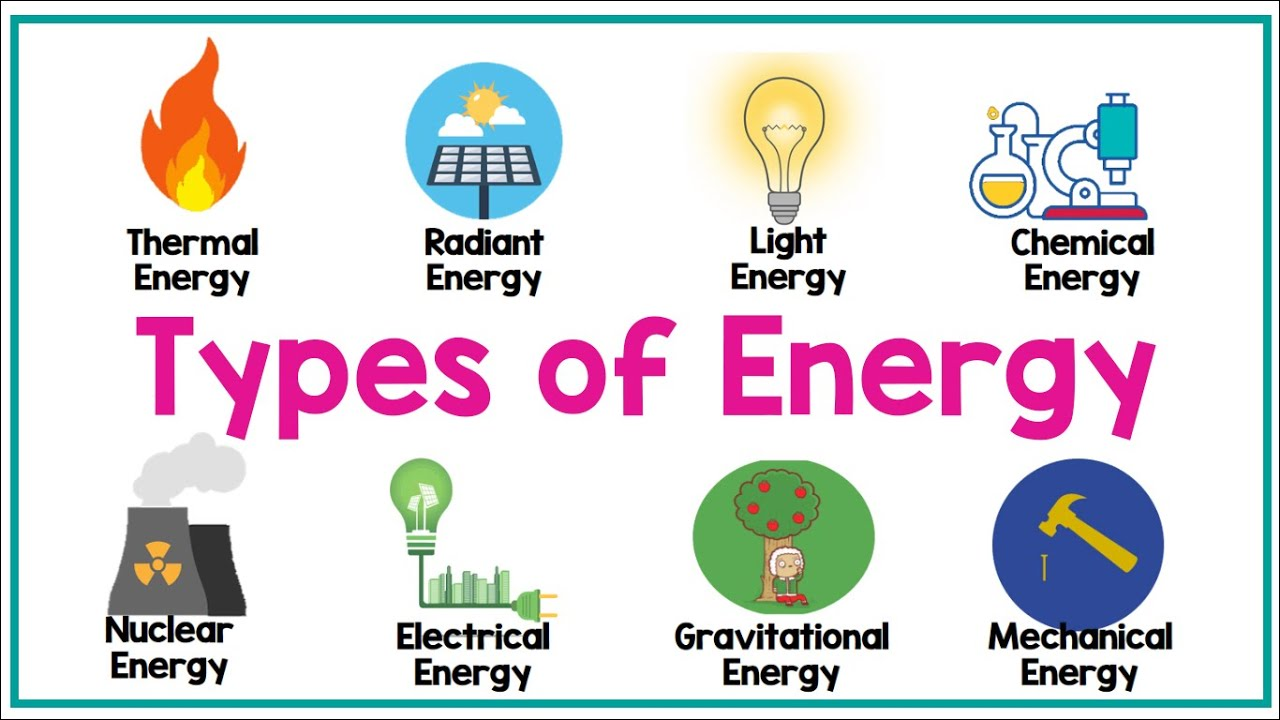
\includegraphics[scale=0.15]{energy_types}
    
    \textbf{Energy is neither created nor destroyed}
  \end{center}

  \begin{itemize}
  \item Energy can be converted from form to another
    e.g. mechanical, chemical, thermal, nuclear,
    electrical and vibrational energy
  \item Converting from one energy form to another is
    never $100\%$ efficient; there is always a loss of
    energy
  \end{itemize}
\end{frame}

\begin{frame}{Context: Energy Loss}
  \centering
  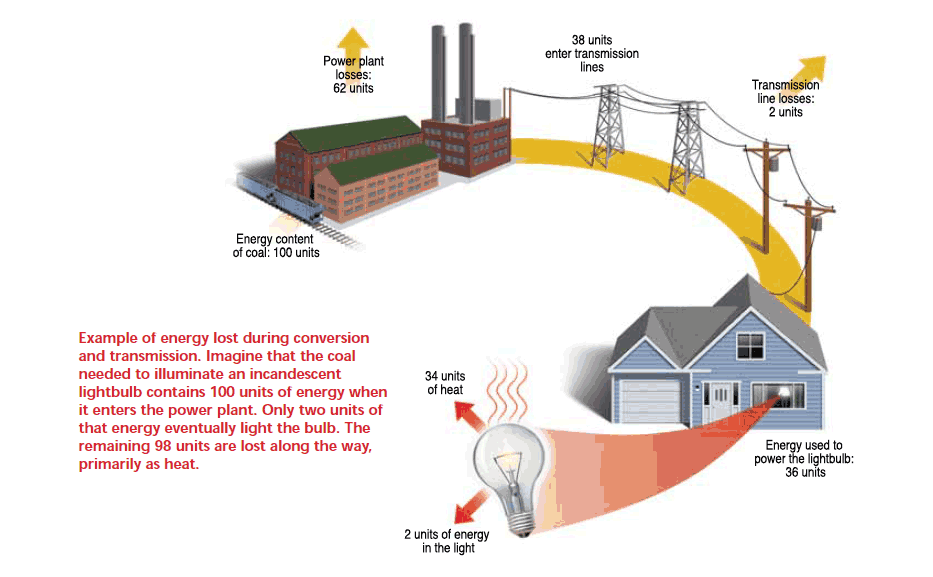
\includegraphics[width=0.9\linewidth]{energy_loss}

  Approximately only $\sim 30\%$ efficiency
\end{frame}

\subsection{Endothermic and Exothermic Reactions}

\begin{frame}{Endothermic and Exothermic Reactions}
  \centering
  
\includegraphics[width=0.8\linewidth]{exo_endo}

  \textbf{Exo} - external; exothermic reactions give off
  heat

  \textbf{Endo} - internal; endothermic reactions absorb
  heat
\end{frame}

\begin{frame}{Endothermic Reaction Diagram}
  \centering
  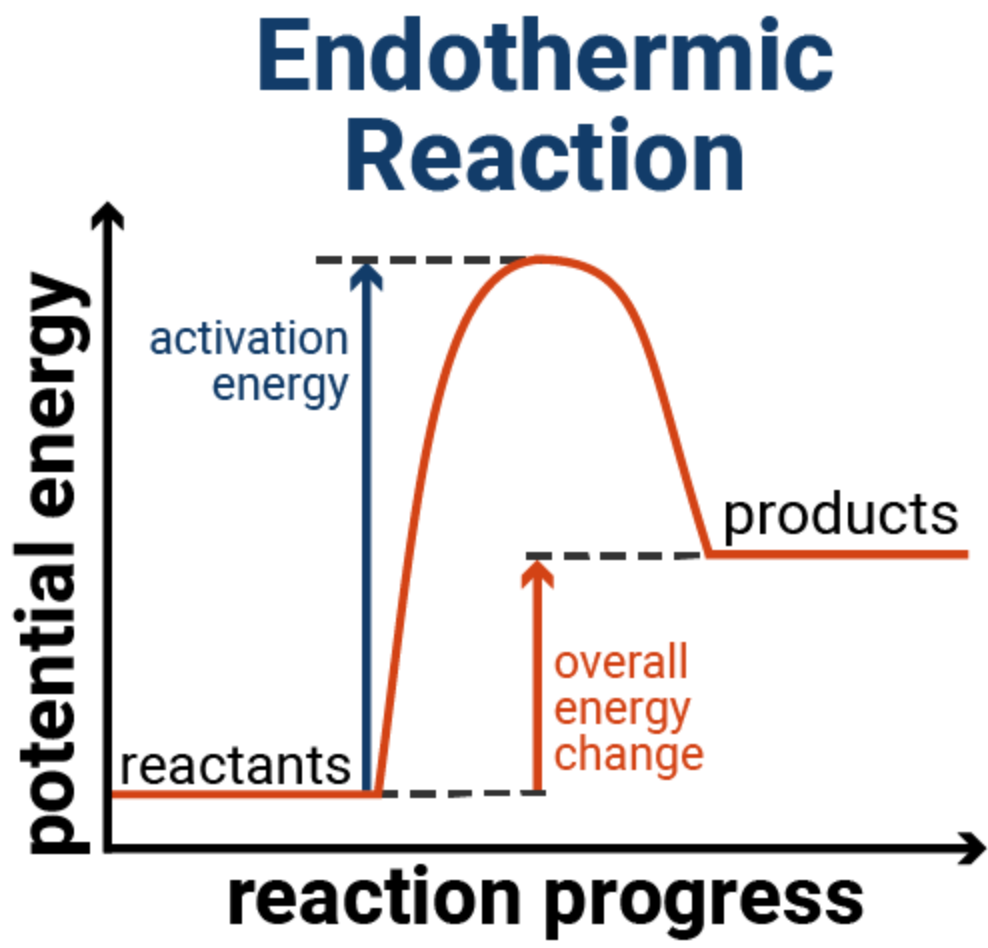
\includegraphics[width=0.5\linewidth]{endo_rxn}

  \begin{itemize}
  \item \textbf{Recall Potential energy} - ability to do
    work; $\Delta E_\text{products} > \Delta E_\text{reactants}$
  \item \textbf{Activation energy} - minimum energy to start the
    reaction; determines the rate at which the reaction undergoes
  \end{itemize}
\end{frame}

\begin{frame}{Examples of Endothermic Reactions}
  \centering
  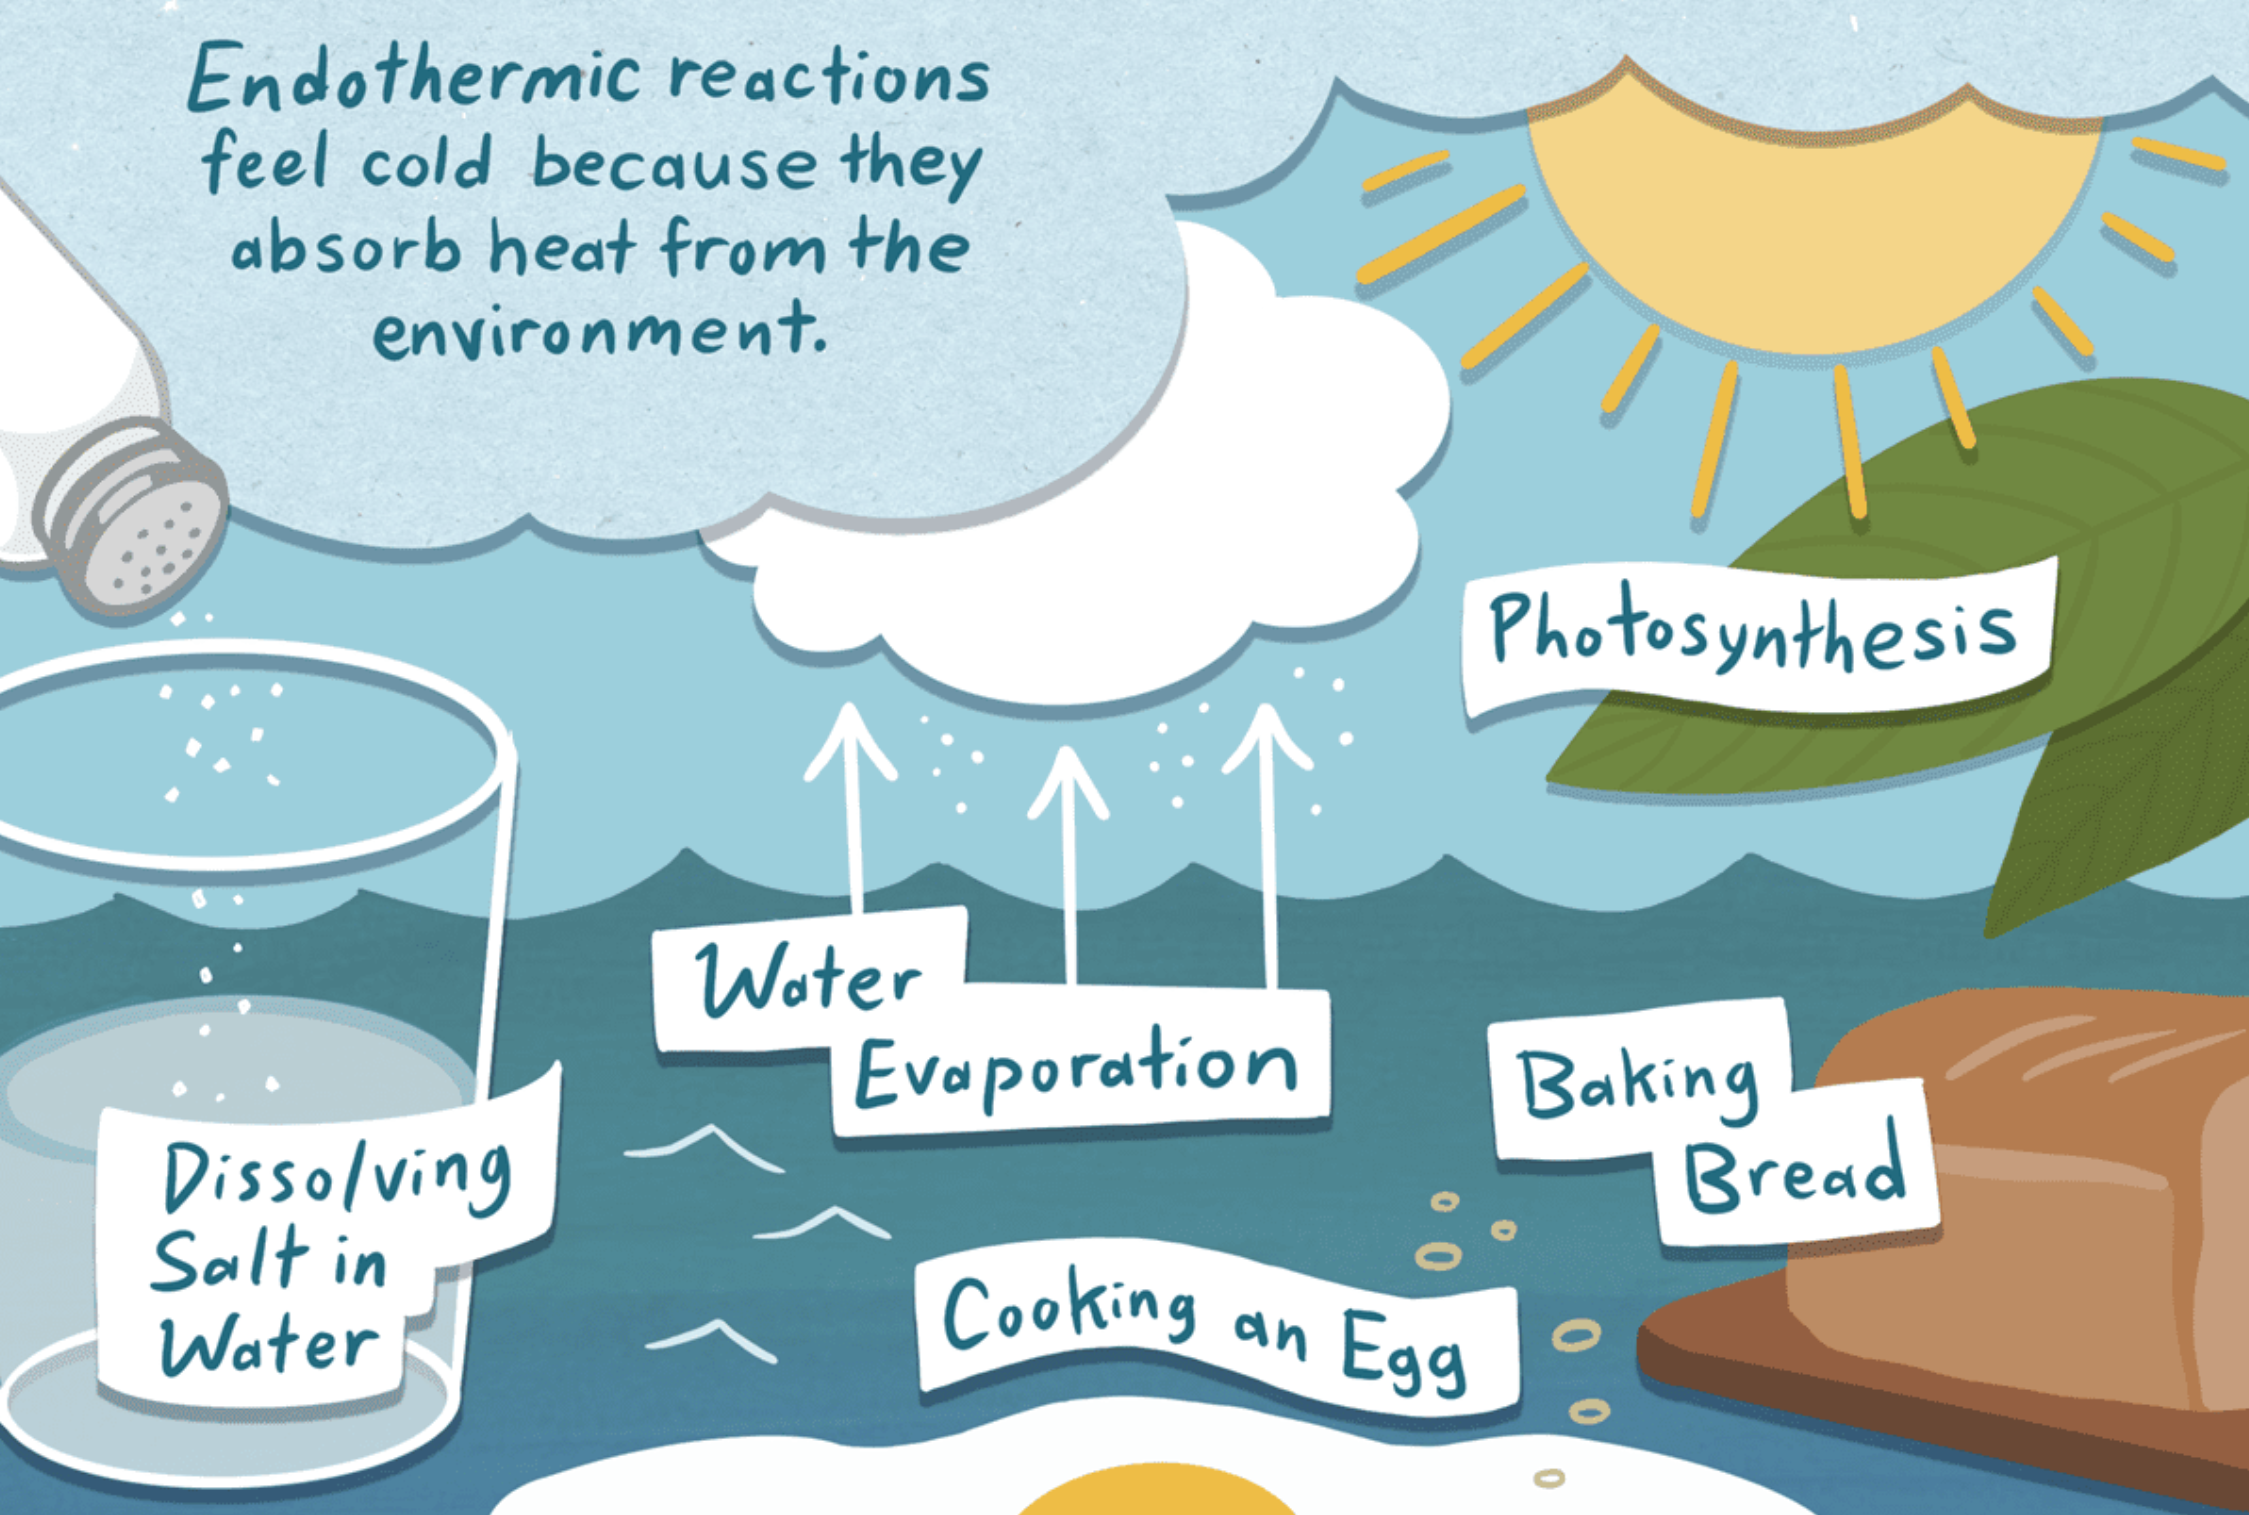
\includegraphics[width=\linewidth]{endo_everyday}
\end{frame}

\begin{frame}{Exothermic Reaction Diagram}
  \centering
  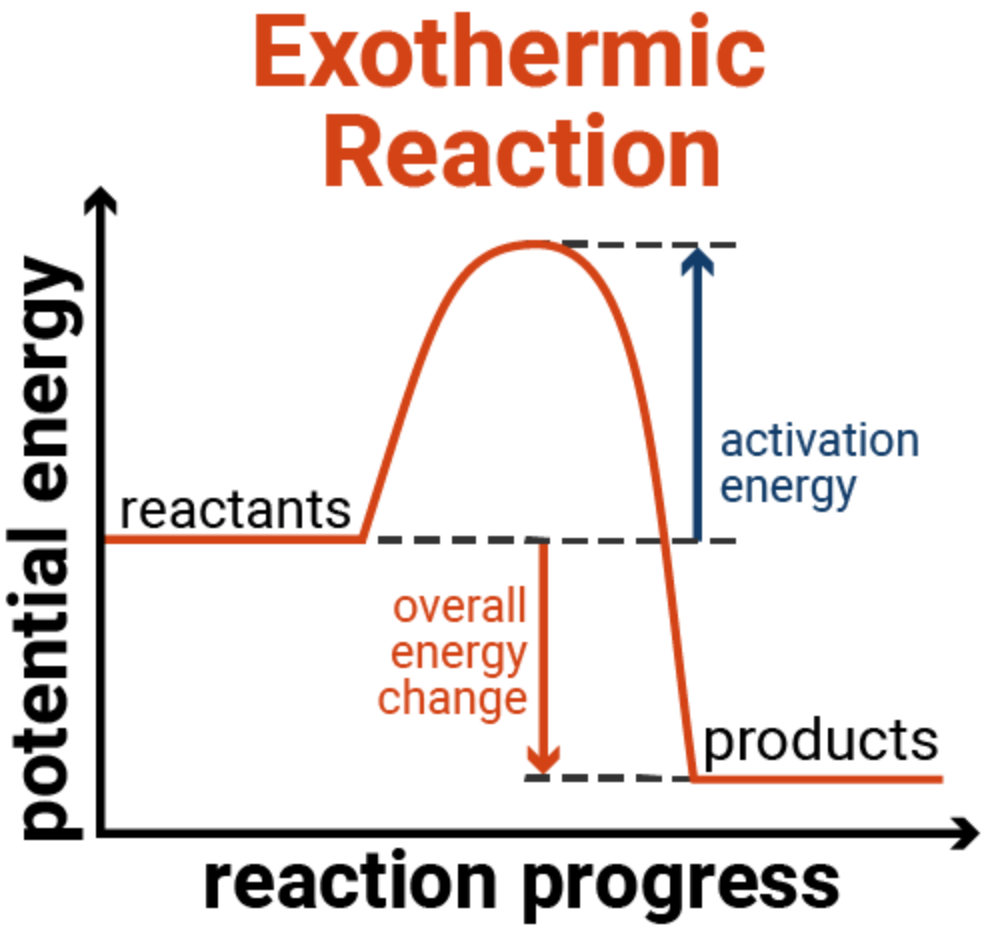
\includegraphics[width=0.5\linewidth]{exo_rxn}
  \begin{itemize}
  \item \textbf{Potential energy} - $\Delta E_\text{products} < \Delta E_\text{reactants}$
  \item Products are more stable than reactants since preference
    for lower energy state
  \end{itemize}
\end{frame}

\begin{frame}{Examples of Exothermic Reactions}
  \centering
  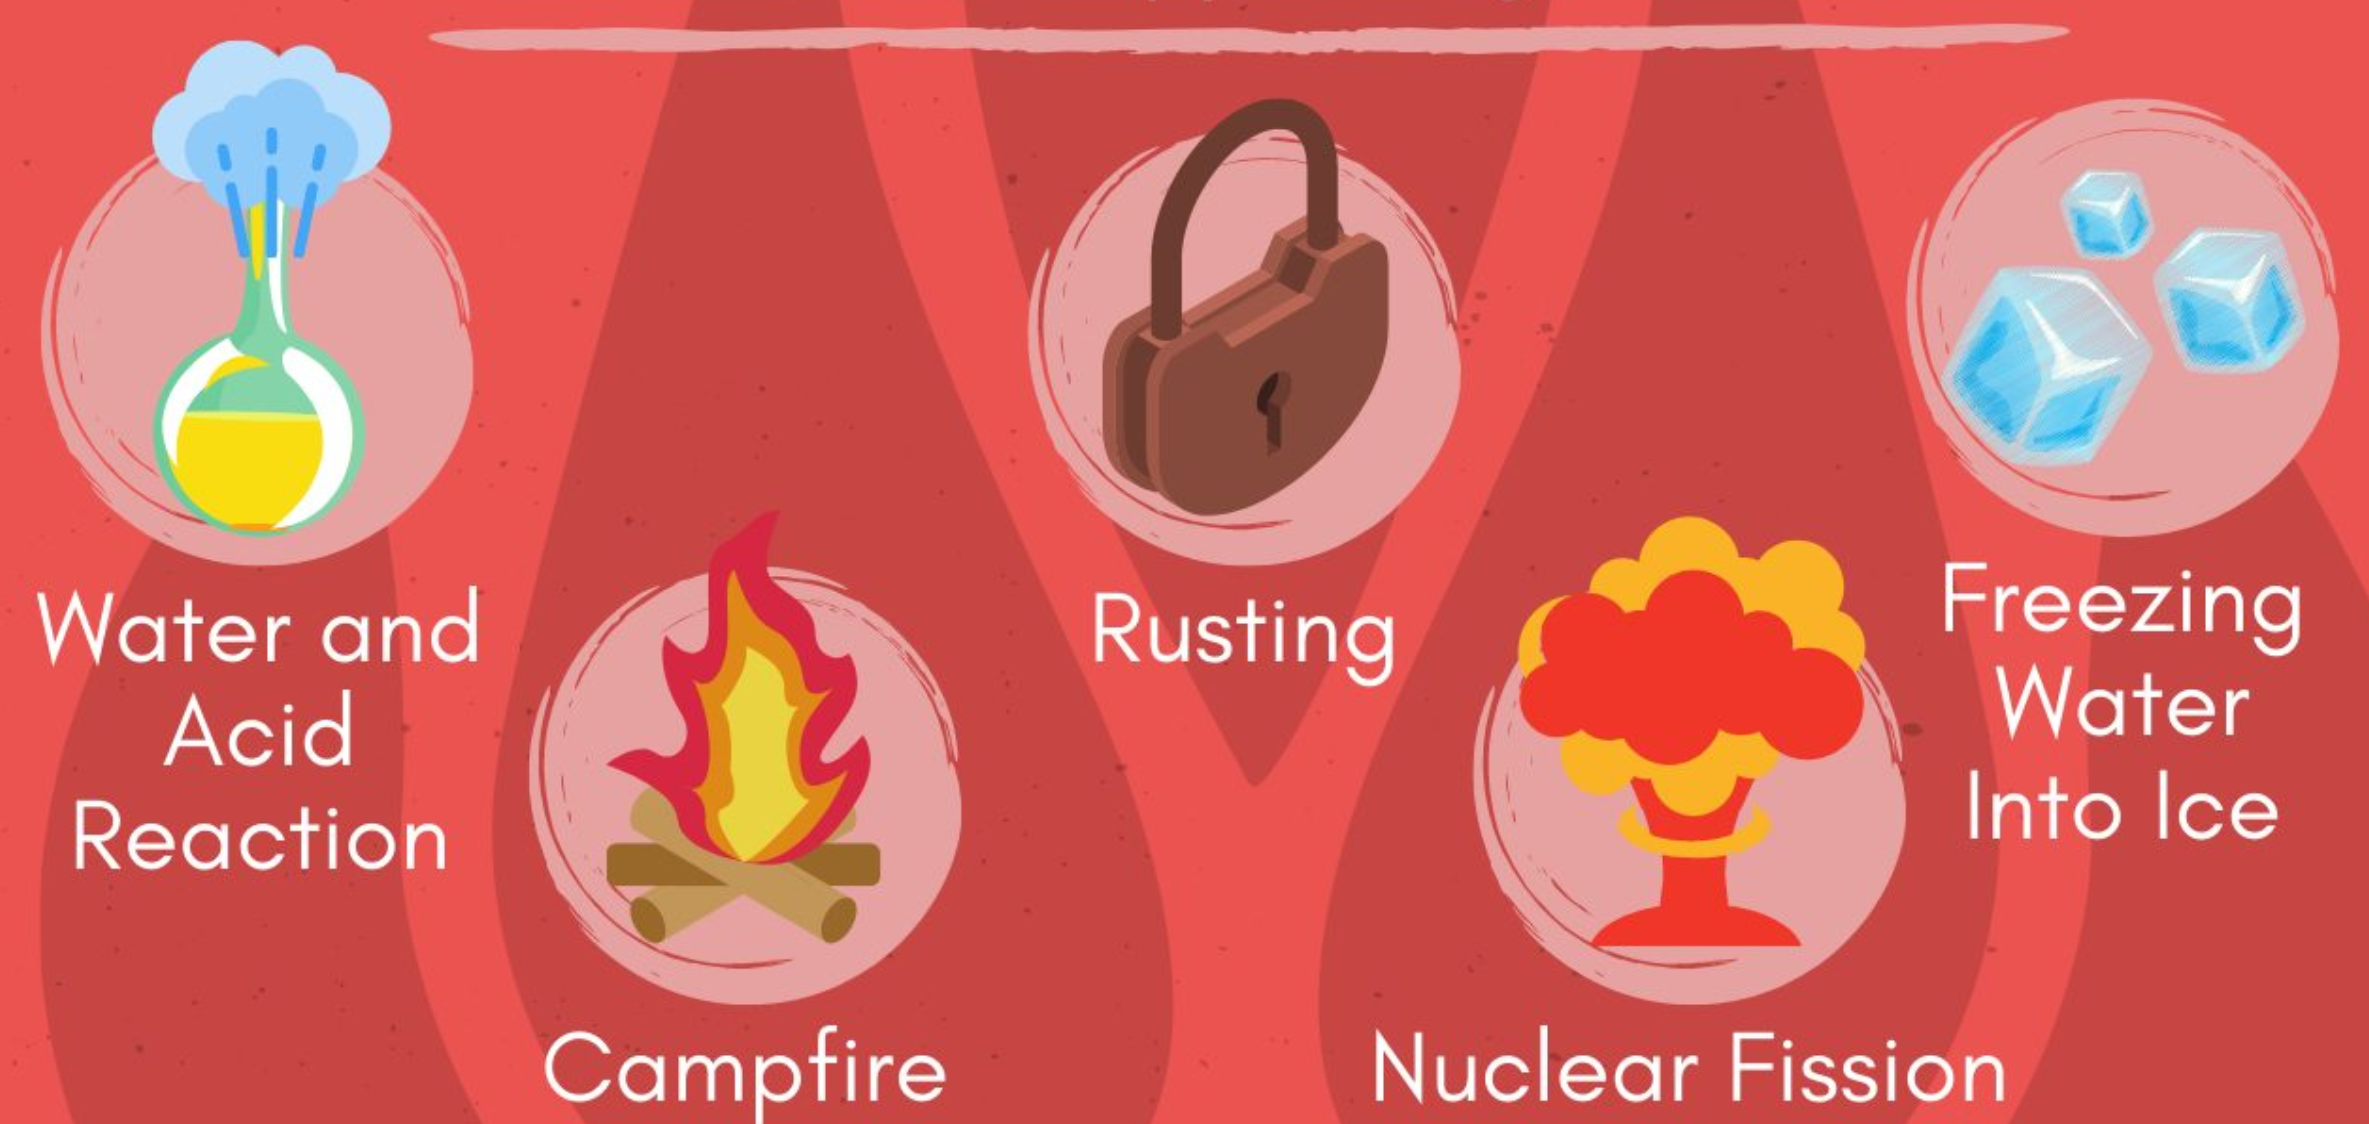
\includegraphics[width=\linewidth]{exo_everyday}
\end{frame}

\begin{frame}{Nuclear Fission}
  \centering
  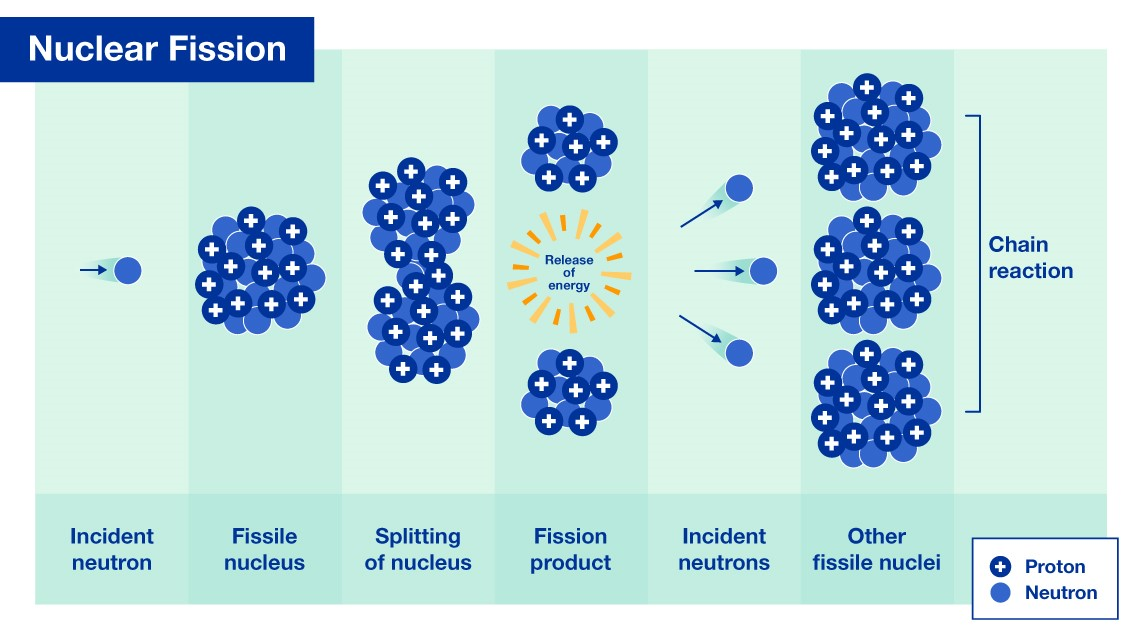
\includegraphics[width=0.8\linewidth]{nuclear_fission}

  \begin{itemize}
  \item \textbf{Nuclear fission} - releases energy where the
    nucleus of an atom splits into two or smaller nuclei
  \item U-235 atoms breaking down to release up to 200 million
    eV ($4.6\times 10^9$ kcal/mol)
  \item \textbf{Context} - 9.71 kcal/mol to boil water
  \end{itemize}
\end{frame}

\subsection{Calorimetry}

\begin{frame}{Calorimetry}
\end{frame}

\end{document}
